% =============================================================================
% Two-column HistoCrypt / proceedings camera-ready style.
% For single-column Cryptologia review submission, replace `twocolumn,10pt`
% with `11pt` and add `\usepackage{setspace}\doublespacing`.
% =============================================================================
\documentclass[10pt,a4paper,twocolumn]{article}

\usepackage{iftex}
\ifPDFTeX
  \usepackage[T1]{fontenc}
  \usepackage[utf8]{inputenc}
\fi
\usepackage[margin=1.60cm,columnsep=0.58cm]{geometry}
\usepackage{lmodern}
\usepackage{microtype}
\usepackage{amsmath,amssymb}
\usepackage{graphicx}
\usepackage{booktabs}
\usepackage{array}
\usepackage{tabularx}
\usepackage{xcolor}
\usepackage{enumitem}
\usepackage[font=small,labelfont=bf,skip=4pt]{caption}
\usepackage[numbers,sort&compress]{natbib}
\usepackage{xurl}
\usepackage[colorlinks=true,linkcolor=navy,citecolor=teal,urlcolor=navy]{hyperref}
\usepackage{titlesec}
\usepackage{fancyhdr}

\definecolor{navy}{HTML}{1E3A5F}
\definecolor{teal}{HTML}{0F766E}
\definecolor{crimson}{HTML}{BE123C}
\definecolor{slate}{HTML}{475569}

\titleformat{\section}{\large\bfseries\color{navy}}{\thesection}{0.6em}{}
\titleformat{\subsection}{\normalsize\bfseries\color{navy}}{\thesubsection}{0.5em}{}
\titlespacing*{\section}{0pt}{9pt plus 2pt minus 2pt}{3.5pt plus 1pt}
\titlespacing*{\subsection}{0pt}{6.5pt plus 1pt minus 1pt}{2.5pt plus 1pt}

\pagestyle{fancy}
\fancyhf{}
\fancyhead[L]{\footnotesize\color{slate}\textit{2D Geometric Signatures and Forensic Corpus Analysis of the Dorabella Cipher (1897)}}
\fancyhead[R]{\footnotesize\color{slate}\thepage}
\renewcommand{\headrulewidth}{0.4pt}
\renewcommand{\headrule}{\hbox to\headwidth{\color{slate!35}\leaders\hrule height \headrulewidth\hfill}}

\setlist[itemize]{leftmargin=1.2em,itemsep=1.5pt,topsep=2.5pt,parsep=0pt}
\setlist[enumerate]{leftmargin=1.4em,itemsep=1.5pt,topsep=2.5pt,parsep=0pt}

\newcommand{\code}[1]{\texttt{\small #1}}

\title{\vspace{-1.0cm}\LARGE\bfseries\color{navy} Two-Dimensional Geometric Signatures, Cross-Corpus Forensic Analysis, and Generative Model Selection for Elgar's Dorabella Cipher (1897)}

\author{%
  \textbf{Christophe Marcheux} \\[2pt]
  \small\color{slate} Independent Researcher \quad$\cdot$\quad Computational assistance credited to Arena.ai Agent Mode (see Acknowledgments) \\
  \small\color{slate} Full code, datasets, and deterministic reproduction pipeline: \code{scripts/reproduce\_all.py}
}

\date{\small November 20, 2026}

\begin{document}

\twocolumn[
\begin{@twocolumnfalse}
\maketitle
\thispagestyle{plain}
\vspace{-0.4cm}
\begin{abstract}
\noindent
Edward Elgar's \emph{Dorabella Cipher} (87 semicircular glyphs arranged in three lines of 29, 31, and 27 symbols, dated ``July 14.~97'') has resisted decipherment since its publication in Dora Powell's memoirs in 1937. While recent cryptanalytic work has established that monoalphabetic substitution cipher (MASC) solvers fail on Dorabella despite achieving 88\%--99\% accuracy on 87-character English and Latin controls \citep{hauer2021dorabella,wase2025dorabella}, permutation-invariant one-dimensional (1D) feature classifiers continue to place Dorabella near the decision boundary between real English and English-like random text \citep{foxon2024ann,foxon2025ml}.

By exploiting the \textbf{two-dimensional (2D) glyph geometry}---eight clockwise orientations in $45^\circ$ increments (\code{A}--\code{H}) paired with 1, 2, or 3 semicircular arcs---rather than abstract symbol identities alone, we uncover \textbf{four robust, empirically weakly correlated 2D signatures} and conduct the \textbf{first systematic quantitative comparison of Elgar's complete surviving semicircle corpus} (1886--1924+):
(1)~\textbf{Dynamic \code{W/V} posture segregation}: orientations split into two $180^\circ$-closed stroke families---cursive waves \code{W=\{B,C,F,G\}} (70.1\%) versus upright/steep strokes \code{V=\{A,D,E,H\}} (29.9\%)---with only $18/86$ cross-group transitions versus $36.46$ expected ($Z = -4.761$, invariant across three independent transcriptions; $0/1{,}000$ English MASC controls reach $\min Z \le -4.76$ across all 35 $4{+}4$ partitions, $p_{\mathrm{corr}} < 0.001$).
(2)~\textbf{Two-layer decomposition of $27/86$ ($31.4\%$) $180^\circ$ flips} ($Z = +4.58$, $p < 2\times 10^{-5}$), resolving Massey (2017) vs.\ Rehling (2020): different-arc $180^\circ$ flips occur equally inside ($8/29 = 27.6\%$) and outside Massey's three non-repeating-arc runs ($p = 0.632$) and are absorbed within fixed \code{W/V} blocks ($p_{\mathrm{intra\text{-}WV}} = 0.221$), whereas same-arc $180^\circ$ flips reach $13/27 = 48.1\%$ ($0/1{,}000$ English MASCs reach $\ge 48.1\%$, $p_{\mathrm{emp}} = 0.001$) and persist even within fixed \code{W/V} blocks and fixed arc positions ($p = 0.0012$; $\mathrm{OR} = 2.99$, $p = 0.044$).
(3)~\textbf{Ergonomic $180^\circ$ arc-profile symmetry}: every orientation and its exact $180^\circ$ opposite share nearly identical arc-count distributions (mean 4-axis cosine $0.9746$, $|\Delta\mathrm{arc}| = 0.1679$, exact rank \textbf{\#1/105} pairings, $p = 0.00952$; $1/1{,}000$ English MASCs reach $\cos \ge 0.9746$, $p_{\mathrm{emp}} = 0.002$; $0/1{,}000$ match all three 2D signatures jointly).
(4)~\textbf{Cross-corpus dissociation}: Elgar's 1886 \emph{Liszt Fragment} ($N=18$) matches Dorabella's marginal profile ($r = +0.750$, $p = 0.032$; \code{W} $= 88.9\%$, peak \code{F}; arcs $\chi^2\,p = 0.881$)---rendering a 1937 forgery by Dora Powell highly implausible---yet displays $0/17$ $180^\circ$ flips, whereas Elgar's post-1924 \emph{Marco Notebook} (verified English ciphertext, $N=39$) diverges sharply (\code{W} $= 41.0\%$, Fisher $p = 0.0029$; $r = -0.342$; arcs $\chi^2\,p = 0.023$).

Leave-one-out cross-validation (LOO-CV) across the 86 orientation transitions confirms that a parsimonious 4-parameter calligraphic model (\code{W/V} posture + $180^\circ$ mirror reflex) gains $+12.03$~nats over independence (Bayes factor $\approx 167{,}000:1$), outperforming a full $8\times 8$ Markov chain ($+7.81$~nats) and an optimal 1D conjunct musical chain ($+8.59$~nats). Finally, augmenting 12 Foxon-style 1D features with our four 2D features lifts RBF-SVM/MLP cross-validation accuracy from $93.4\%$ to $99.94\%$ ($\mathrm{AUC}=0.9999$): Dorabella flips from $P(\mathrm{English}\mid\mathrm{1D}) = 0.772/0.973$ to $P(\mathrm{English}\mid\mathrm{1D{+}2D}) = 0.0008/0.0016$ across all three transcriptions, while Elgar's real \emph{Marco Notebook} ciphertext moves in the opposite direction to $P(\mathrm{English}\mid\mathrm{1D{+}2D}) = 1.0000$.
\end{abstract}
\vspace{0.25cm}
\noindent\textbf{\small Keywords:} {\small Dorabella Cipher; Edward Elgar; Historical Cryptology; 2D Glyph Geometry; Hoax Cryptogram Detection; Model Selection; Reproducible Analysis.}
\vspace{0.35cm}
\end{@twocolumnfalse}
]

% =============================================================================
\section{Introduction and Prior-Art Audit}
\label{sec:intro}
% =============================================================================

Sent by the British composer Edward Elgar to twenty-two-year-old Dora Penny on 14 July 1897 and first published forty years later in her memoirs \citep{powell1937memories}, the \emph{Dorabella Cipher} consists of 87 calligraphic symbols written in three lines (29, 31, and 27 glyphs) using an alphabet of 1, 2, or 3 connected semicircles oriented along eight compass directions. Despite numerous proposed plaintexts \citep[e.g.,][]{sams1970dorabella}, no decipherment has achieved consensus.

Over the past decade, computational cryptology has sharply narrowed the hypothesis space. \citet{schmeh2018dorabella} demonstrated the failure of classical vowel/consonant-line identification and noted an elevated count of reversed digrams ($12$, twice a contemporary English control). \citet{hauer2021dorabella} showed that five state-of-the-art MASC solvers fail to produce coherent English on Dorabella despite solving 88.1\% of 87-character English controls; \citet{wase2025dorabella} independently confirmed with CrypTool~2 that 98.7\% of English and 98.6\% of Latin 87-character MASCs are solved while Dorabella and simple permutations resist decipherment.\footnote{\textbf{Bibliographic transparency note:} Because \citet{wase2025dorabella} (published online Nov.\ 2023, print Jan.\ 2025, DOI~\code{10.1080/01611194.2023.2271466}) is behind a publisher paywall with no open preprint, verification relies on its official abstract, keyword metadata (\code{CrypTool 2}), and secondary citations \citep{foxon2024ann}. Direct verification against the publisher PDF is recommended prior to archival publication.} Simultaneously, \citet{foxon2024ann,foxon2025ml} trained neural and SVM hoax-detection classifiers on 15 permutation-invariant 1D symbol statistics, finding that Dorabella receives high English-class probabilities (NN $0.75$, SVM $0.81$) yet sits on the manifold boundary between real English and English-like random text---leading \citet{foxon2025ml} to explicitly call for new discriminating features.

A parallel strand of forensic scholarship has examined the visual appearance of the cipher. \citet{massey2017dorabella} identified three long runs without consecutive arc-count repetitions near the start of each line (13, 10, and 9 glyphs in consensus transcription) and 13 adjacent same-arc $180^\circ$ mirror pairs, arguing that Dorabella is a friendly hoax. \citet{pelling2019dorabella} and commenters documented J.~Rehling's objection that non-repeating-arc runs and same-arc mirror pairs are mutually exclusive by construction. \citet{hauer2021dorabella} confirmed that 13 same-arc mirrors are rare in English MASCs ($123/100{,}000$, $p \approx 0.0012$, mean $3.64$), while showing that Massey's length-12 arc run is unremarkable in English ($27.4\%$). Meanwhile, T.~Ernst \citep[summarized in][]{schmeh2021faelschung} tabulated marginal angle-by-arc preferences and proposed a 1937 forgery by Dora Powell, while \citet{pelling2019dorabella} remarked on line-3 monotony and suggested comparing Dorabella with Elgar's 1886 \emph{Liszt Fragment}.

Table~\ref{tab:priorart} delimits rigorously what was previously established from the novel quantitative contributions introduced in this paper.

\begin{table*}[t]
\centering
\caption{Strict prior-art audit separating established findings, qualitative remarks, and novel quantitative contributions of this study.}
\label{tab:priorart}
\footnotesize
\renewcommand{\arraystretch}{1.12}
\begin{tabularx}{\textwidth}{@{}p{4.3cm} c X@{}}
\toprule
\textbf{Finding / Feature} & \textbf{Prior Status} & \textbf{Exact References and Scope of Present Contribution} \\
\midrule
MASC solver failure (EN/LA, $N=87$) & Established & \citet{hauer2021dorabella} (88.1\% EN controls); \citet{wase2025dorabella} (98.7\% EN, 98.6\% LA). \emph{Added here:} 5 languages (\code{EN, IT, DE, FR, GA}), 5 phonetic/shorthand regimes, backslang, 4 transcriptions + $2^5$ visual flips, and $180^\circ$ flip ciphers (\code{F1--F4}). \\
13 same-arc $180^\circ$ mirror pairs & Established & \citet{massey2017dorabella}; binomial correction by Rehling \citep{pelling2019dorabella}; \citet{hauer2021dorabella} (\S6.4.1, $p\approx 0.0012$). \emph{Added here:} refutation of double-letter and $180^\circ$-flip mechanisms (\code{M1--M2}, \code{F1--F4}) + EN MASC rate null ($0/1{,}000$). \\
Non-repeating-arc runs ($13,10,9$) & Established & \citet{massey2017dorabella}; Jarlve (Liszt run of 8--9) \& Rehling (mutual exclusivity) in \citet{pelling2019dorabella}; \citet{hauer2021dorabella} (\S6.4.2, 27.4\% in EN MASC). \emph{Added here:} proves this feature strongly rejects tested pitch+rhythm Elgar music encodings ($+9.2\sigma$). \\
12 reversed digrams (\code{RevD}=12) & Established & \citet{schmeh2018dorabella} (\S3.5, p.~148; $2\times$ 1897 English control). \\
Angle bias \& L3 visual monotony & Qualitative & \citet{ernst2018cipherbrain} in \citet{schmeh2021faelschung} (marginal Angle$\times$Arcs table); \citet{pelling2019dorabella} (L3 monotony, Liszt comparison suggested). \emph{Added here:} formal dynamic \code{W/V} test, exact symmetry rank, and cross-corpus tests. \\
Identical L1/L2 ending (\code{B3 F3}) & Partial & R.~Novacna \citep{pelling2019dorabella} and \citet{hauer2021dorabella} (\S6.4.1). \emph{Added here:} exploratory look-elsewhere calibration of \code{lag=31} ($11/56$) and late L1/L2 12-glyph window ($6/12$). \\
Marco notebook $8!\times 2$ key space & Established & \citet{amreshra2024dorabellalab} (80,640 permutations + keywords). \emph{Added here:} 72,960 geometric/rotating-pigpen/card keys. \\
1D ML hoax classification & Established & \citet{foxon2024ann,foxon2025ml} (15 1D features; calls for new discriminating features). \emph{Added here:} direct 1D vs.\ 1D+2D SVM/MLP validation resolving the boundary on Dorabella and Marco. \\
\midrule
\textbf{\code{W/V} posture blocks ($Z=-4.76$), two-layer $27/86$ $180^\circ$ flips, $180^\circ$ arc-profile symmetry (\#1/105), 1,000 EN MASC 2D nulls, Liszt--Dorabella--Marco corpus tests, LOO-CV \& 1D+2D classifier} & \textbf{Novel} & \textbf{Original quantitative contributions of this study (100\% deterministically reproducible via \code{scripts/reproduce\_all.py}).} \\
\bottomrule
\end{tabularx}
\end{table*}

% =============================================================================
\section{Data, Conventions, and Methodology}
\label{sec:methods}
% =============================================================================

\subsection{Glyph Coding and Multi-Transcription Controls}
Each semicircle glyph is represented as an ordered pair $(o, a) \in \{\code{A},\dots,\code{H}\}\times\{1,2,3\}$, where $o$ denotes clockwise orientation in $45^\circ$ steps starting from an upright right-opening $\varepsilon$ (\code{A} $= 0^\circ$, \code{B} $= 45^\circ$, \code{C} $= 90^\circ$, \code{D} $= 135^\circ$, \code{E} $= 180^\circ$, \code{F} $= 225^\circ$, \code{G} $= 270^\circ$, \code{H} $= 315^\circ$) and $a$ is the number of connected semicircular arcs. Direct inspection of Elgar's undated \emph{Cryptogram Card} \citep{bauer2017unsolved} confirms that this clockwise $45^\circ$ cycle is Elgar's own enumeration order (\code{A3 B3 C3 D3 E3 F3 G3 H3 A2 A1}, followed by \code{A3 A2 A1 B3 B2 B1}), establishing the card as an alphabet specimen rather than a ciphertext.

To guarantee that no geometric signature is an artifact of subjective glyph reading, every core test is replicated across \textbf{three independent oriented transcriptions} stored in \code{data/transcriptions.json}: \code{Hauer\_2025} (five-source consensus \citep{hauer2025dorabella}; 20 unique glyphs, $\mathrm{IC} = 0.05854$, $\mathrm{Dbl} = 4$, $\mathrm{RevD} = 12$), \code{Hartmeier\_2017} \citep{hartmeier2017dorabella}, and \code{Pelling\_2012} \citep{pelling2019dorabella}.

\subsection{Elgar's Complete Surviving Semicircle Corpus}
Stored in \code{data/elgar\_corpus.json}, our cross-document analysis covers all three surviving Elgar manuscripts employing this alphabet:
\begin{enumerate}
  \item \textbf{\emph{Liszt Fragment} (10 April 1886, $N=18$):} Marginal pencil note written on a Crystal Palace concert programme alongside Liszt's \emph{Les Pr\'eludes}, held at the Elgar Birthplace Museum \citep{bauer2017unsolved}. We analyze both our visually verified standard reading (\code{Liszt\_1886\_std}) and a three-glyph tilt-sensitivity variant (\code{Liszt\_1886\_alt}: \code{\#8=H2}, \code{\#15=E3}, \code{\#18=H1}).
  \item \textbf{\emph{Dorabella Cipher} (14 July 1897, $N=87$):} Three lines (29, 31, 27 glyphs) with a single medial dot after \code{L3\#5}.
  \item \textbf{\emph{Marco Elgar Notebook} (post-May 1924, $N=39$ and $N=47$):} Held at the Elgar Birthplace Museum and dated after the birth of Elgar's spaniel Marco (27 May 1924), containing an explicit key (\code{ABC / DEF / GHIJ / KLM / NOP / QRS / TUVW / XYZ} mapped to \code{A..H}) and verified English ciphertexts (\code{MARCO ELGAR}, \code{A VERY OLD CYPHER}, \code{DO YOU GO TO LONDON} [$N=39$], plus \code{TOMORROW} [$N=47$]).
\end{enumerate}

\subsection{Summary of Prior Cryptanalytic Refutations}
Before modeling 2D calligraphic dynamics, eight calibrated cryptanalytic scripts (archived in \code{cipher\_refutation/}) systematically ruled out classical and exotic textual hypotheses on $N=87$ controls: MASC plus transpositions across five languages (\code{EN, IT, DE, FR, GA} 18- and 23-letter alphabets), four transcriptions and $2^5 = 32$ disputed visual flips; five phonetic/shorthand encodings and word-level backslang; polyalphabetic periods $p=2..15$, Nihilist $3\times 8$, 23,808 Vigen\`ere/Beaufort/Autokey keys, depth $3\times 31$, $3\times 8$ fractionation, Bifid $5\times 5$, and 72,960 geometric/rotating-pigpen variants of the 1924 key; and four $180^\circ$-inversion cipher mechanisms (\code{F1}--\code{F4}). Across all families, Dorabella's best language-model scores ($-245.1$ to $-217.4$) remain indistinguishable from random negative controls ($-245.1 \pm 2.2$) and far below positive 87-character English controls ($-188.6$ to $-186.5$).

% =============================================================================
\section{2D Geometric Signatures of Dorabella}
\label{sec:results2d}
% =============================================================================

Figure~\ref{fig:map} presents a unified 2D structural map of the 87 glyphs of Dorabella, showing how posture blocks, Massey's non-repeating-arc runs, both layers of $180^\circ$ flips, and the exploratory late L1/L2 \code{lag=31} echo interlock across the three lines.

\begin{figure*}[t]
  \centering
  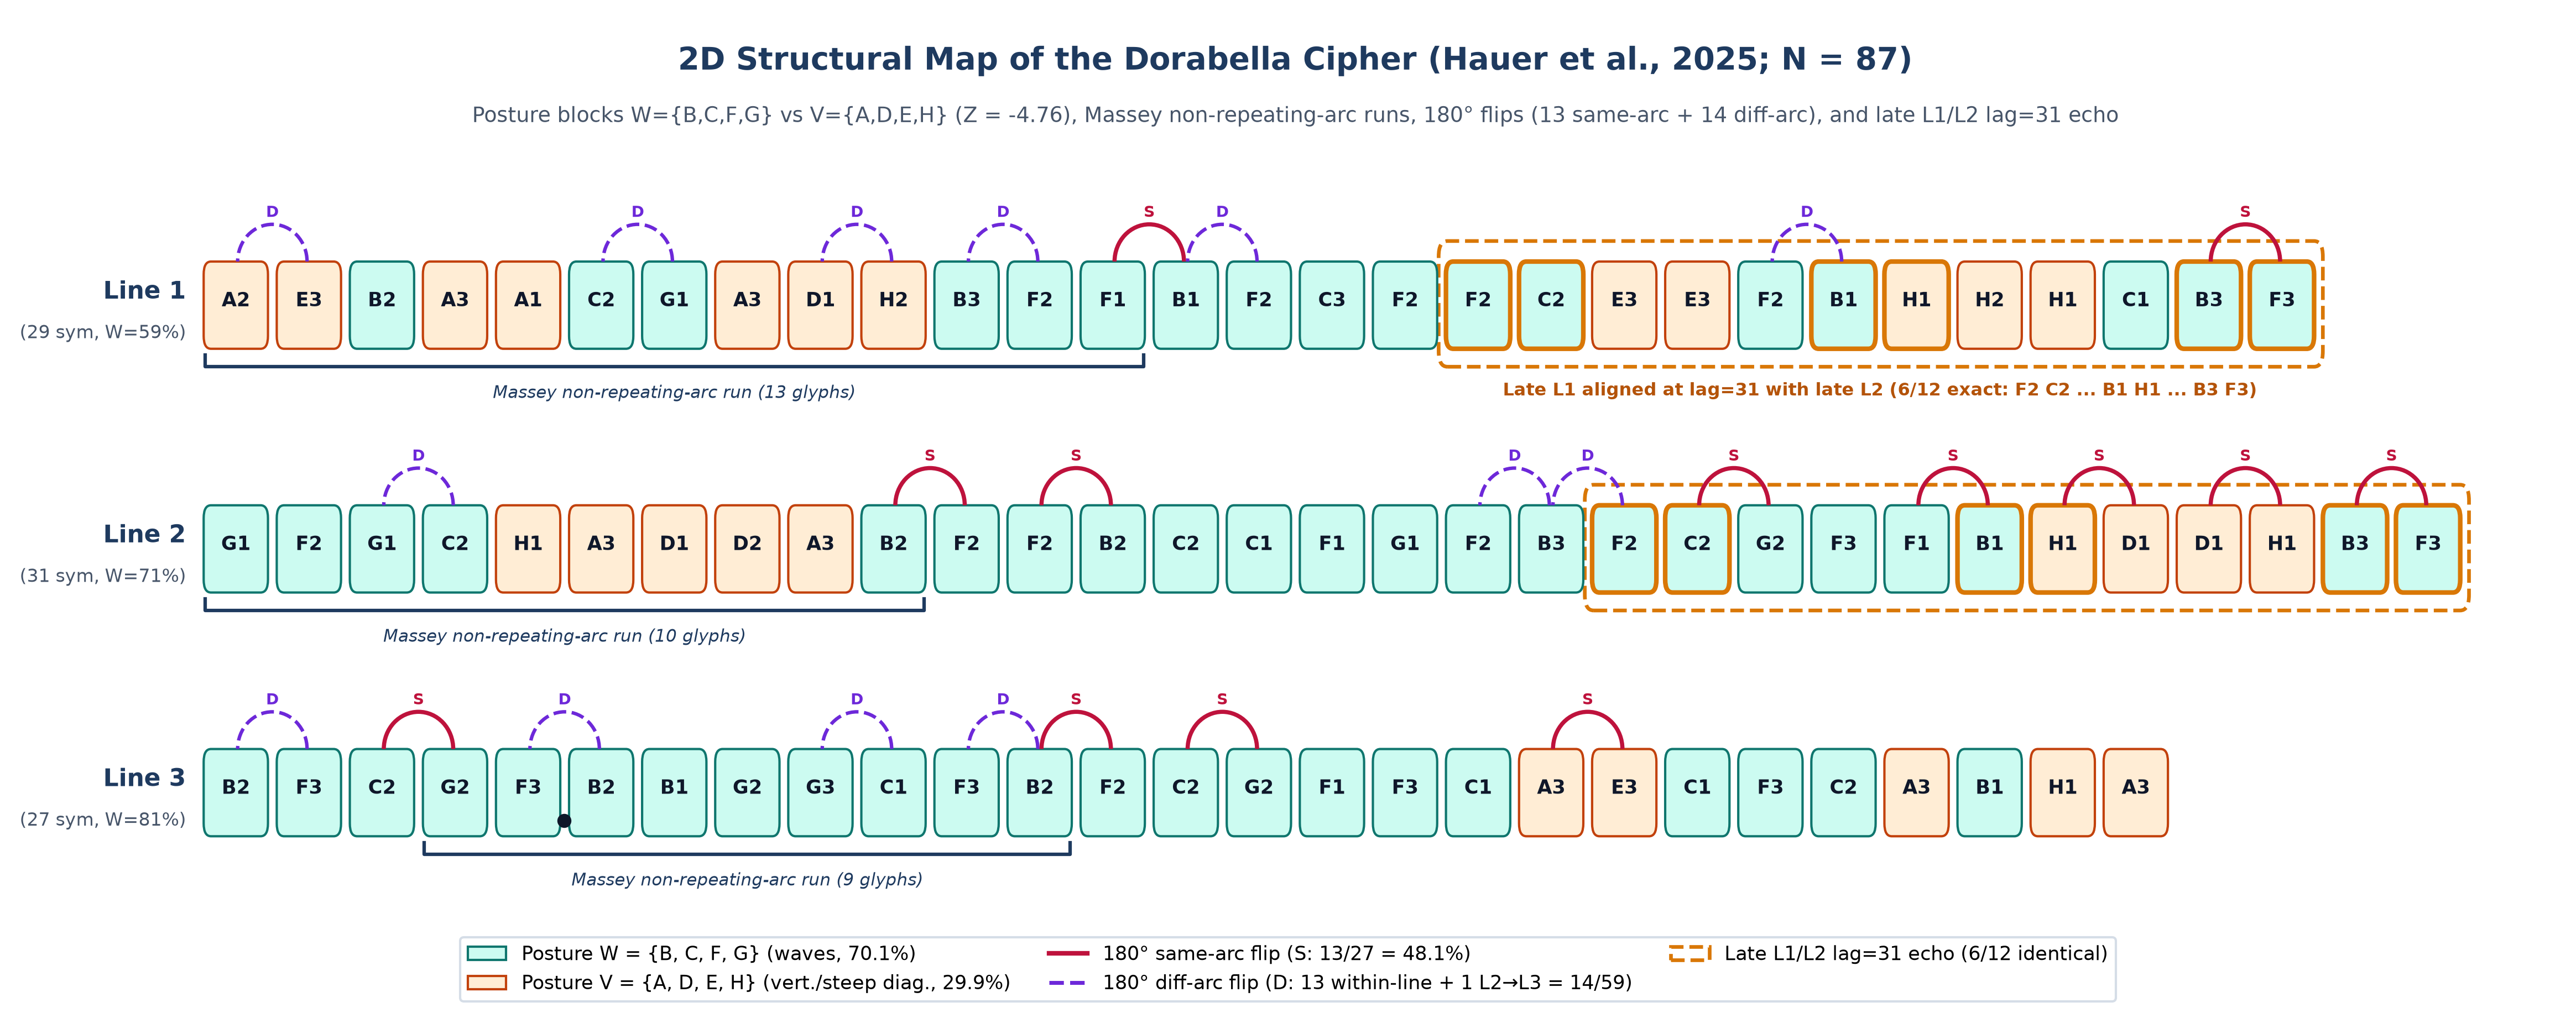
\includegraphics[width=\textwidth]{figures/fig1_en.png}
  \caption{Complete 2D structural map of the Dorabella Cipher (\code{Hauer\_2025}, $N=87$). Teal tiles mark cursive-wave posture \code{W=\{B,C,F,G\}} (70.1\%); amber tiles mark upright/steep posture \code{V=\{A,D,E,H\}} (29.9\%). Solid crimson arcs (\code{S}) denote $180^\circ$ same-arc flips ($13/27 = 48.1\%$); dashed purple arcs (\code{D}) denote $180^\circ$ different-arc flips ($13$ within-line plus $1$ across \code{L2}$\to$\code{L3}, totaling $14/59$). Brackets beneath each line mark Massey's non-repeating-arc runs ($13, 10, 9$ glyphs); dashed gold boxes highlight the exploratory late L1/L2 \code{lag=31} echo ($6/12$ identical glyphs).}
  \label{fig:map}
\end{figure*}

\subsection{Macroscopic \code{W/V} Posture Segregation}
Partitioning the eight compass orientations by pen posture yields two equal-sized classes of four orientations that are \textbf{both closed under $180^\circ$ rotation} (\code{B}$\leftrightarrow$\code{F}, \code{C}$\leftrightarrow$\code{G} inside \code{W}; \code{A}$\leftrightarrow$\code{E}, \code{D}$\leftrightarrow$\code{H} inside \code{V}):
\begin{itemize}
  \item \textbf{Wave posture \code{W=\{B,C,F,G\}}} ($61/87 = 70.1\%$): horizontal and forward-slanted cursive waves (\code{m}, \code{w}) aligned with natural right-handed handwriting flow;
  \item \textbf{Vertical/steep posture \code{V=\{A,D,E,H\}}} ($26/87 = 29.9\%$): upright (\code{$\varepsilon$}, \code{3}) and steep diagonal strokes requiring a wrist-posture change.
\end{itemize}

Along the cipher, \code{W} and \code{V} segregate into long homogeneous runs---up to 16 consecutive \code{W} glyphs in L2, 18 in L3, and 20 across the \code{L2}$\to$\code{L3} line break:
\begin{quote}\footnotesize\ttfamily\noindent
L1 (29): VVWVVWWVVVWWWWWWWWWVVWWVVVWWW\\
L2 (31): WWWWVVVVVWWWWWWWWWWWWWWWWVVVVWW\\
L3 (27): WWWWWWWWWWWWWWWWWWVVWWWVWVV
\end{quote}

Across all 86 transitions, only \textbf{18 cross between \code{W} and \code{V}}, compared to $36.46 \pm 3.88$ expected under random permutation (\textbf{$Z = -4.761$}). Table~\ref{tab:wv} confirms complete invariance across all three transcriptions.

\begin{table}[t]
\centering
\caption{Invariance of \code{W/V} posture segregation and conditional \code{F}$\leftrightarrow$\code{V} boundary avoidance across three transcriptions.}
\label{tab:wv}
\scriptsize
\setlength{\tabcolsep}{3pt}
\resizebox{\columnwidth}{!}{%
\begin{tabular}{@{}lcccc@{}}
\toprule
\textbf{Transcription} & \textbf{\code{W} (\%)} & \textbf{Crossings (exp.)} & \textbf{$Z_{WV}$} & \textbf{\code{F}$\leftrightarrow$\code{V} (uncond.\ $p$)} \\
\midrule
\code{Hauer\_2025}     & 61 (70.1\%) & \textbf{18/86} (36.46) & \textbf{$-4.761$} & 1/46 ($<2\times 10^{-5}$) \\
\code{Hartmeier\_2017} & 62 (71.3\%) & \textbf{18/86} (35.63) & \textbf{$-4.655$} & 1/46 ($<2\times 10^{-5}$) \\
\code{Pelling\_2012}   & 61 (70.1\%) & \textbf{18/86} (36.46) & \textbf{$-4.761$} & 0/42 ($<2\times 10^{-5}$) \\
\bottomrule
\end{tabular}}
\end{table}

\textbf{Look-elsewhere correction across all 35 $4{+}4$ partitions:} Because \code{W/V} was identified empirically rather than pre-registered, rigorous multiple-testing correction over all $\frac{1}{2}\binom{8}{4}=35$ splits is essential. \code{W/V} stands out sharply (Figure~\ref{fig:geom}A): the second-most segregated split (\code{\{C,E,F,G\}} vs.\ \code{\{A,B,D,H\}}, $Z = -3.21$) and ranks \#3--\#5 ($Z = -2.33, -2.27, -1.96$) all share 3 of 4 orientations with \code{W/V} and are \emph{not} closed under $180^\circ$ rotation, confirming that \code{W/V} is the sole $180^\circ$-closed parent behind the tail. Evaluating the \emph{minimum} $Z$ across all 35 partitions on \textbf{1,000 English MASC controls} ($N=87$) yields a mean minimum of $-1.805 \pm 0.620$, a worst observed value of $-4.052$, and \textbf{$0/1{,}000$} controls reaching $\le -4.76$ ($p_{\mathrm{corr}} < 0.001$). Crucially, because both \code{W} and \code{V} are closed under $180^\circ$ rotation, \textbf{no $180^\circ$-flip cryptosystem can either create or erase this block structure}.

\textbf{Conditional \code{F}$\leftrightarrow$\code{V} boundary avoidance (non-double-counted):} Although unconditional \code{F}$\leftrightarrow$\code{V} avoidance ($1/46$) partly reflects \code{F}'s modal status inside \code{W}, conditioning strictly on the 18 fixed \code{W}$\leftrightarrow$\code{V} boundary edges (50,000 permutations of \code{F} within fixed \code{W} positions) still yields $1$ observed boundary contact versus $6.80 \pm 1.99$ expected ($69/50{,}000$, $p = 0.0014$), showing that \code{F} preferentially occupies the interior of \code{W} blocks. To avoid double-counting, we treat this as a structural refinement of \code{W/V} rather than an independent signature.

\begin{figure*}[t]
  \centering
  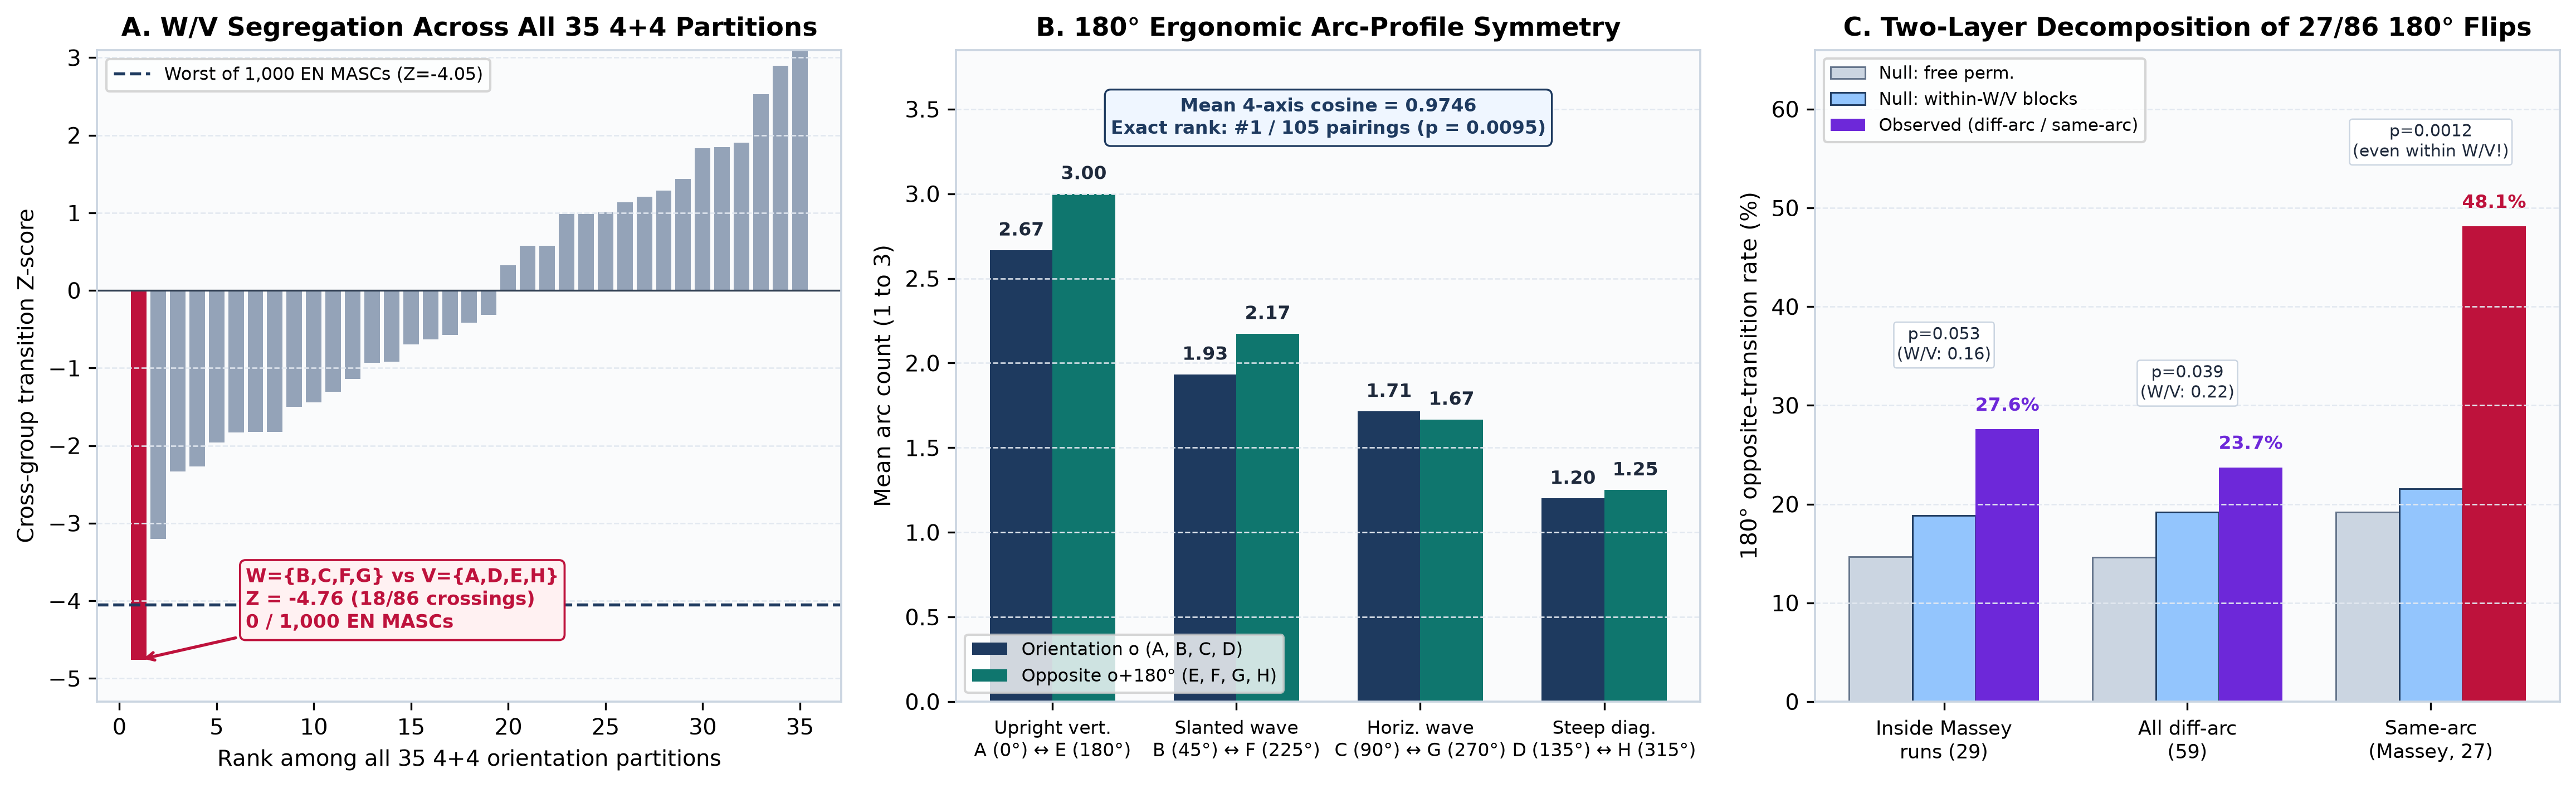
\includegraphics[width=\textwidth]{figures/fig2_en.png}
  \caption{Three core 2D geometric signatures of Dorabella (\code{Hauer\_2025}). \textbf{(A)}~Cross-group transition $Z$-scores across all 35 $4{+}4$ orientation partitions: \code{W=\{B,C,F,G\}} vs.\ \code{V=\{A,D,E,H\}} stands at $Z = -4.76$, well below the worst of 1,000 English MASC controls ($Z = -4.05$). \textbf{(B)}~Mean arc counts along the four $180^\circ$ opposite axes: mean 4-axis cosine $= 0.9746$, exact rank \#1/105 pairings ($p = 0.0095$; $1/1{,}000$ English MASCs). \textbf{(C)}~Two-layer decomposition of the $27/86$ $180^\circ$ transitions against free permutation and within-\code{W/V} permutation nulls.}
  \label{fig:geom}
\end{figure*}

\subsection{Two-Layer Decomposition of $27/86$ $180^\circ$ Flips: Resolving Massey vs.\ Rehling}
Generalizing Massey's 13 same-arc mirror pairs to \emph{all} adjacent $180^\circ$ opposite orientations regardless of arc count doubles the signal to \textbf{$27/86$ ($31.4\%$)} on \code{Hauer\_2025} ($26$ within-line plus \code{L2\#31$\to$L3\#1}: \code{F3$\to$B2}), against $12.57 \pm 3.16$ expected under free permutation ($Z = +4.58$, $p < 2\times 10^{-5}$; \code{Hartmeier\_2017}: $29/86$, $Z = +5.01$; \code{Pelling\_2012}: $26/86$, $Z = +4.22$).

Stratifying these 27 flips by arc-count equality and by Massey's three non-repeating-arc runs ($29$ transitions total, all necessarily different-arc) cleanly resolves the controversy between \citet{massey2017dorabella} and Rehling \citep{pelling2019dorabella} (Table~\ref{tab:flips} and Figure~\ref{fig:geom}C):
\begin{enumerate}
  \item \textbf{Layer 1 (Posture confinement):} Rehling is right that the absence of \emph{same-arc} mirrors during the opening of each line is an artifact of mutual exclusivity---different-arc $180^\circ$ flips begin at the very first transition (\code{A2$\to$E3}) and occur at an indistinguishable rate \emph{inside} Massey's runs ($8/29 = 27.6\%$; $9/29 = 31.0\%$ in Hartmeier) and outside ($19/57 = 33.3\%$; Fisher $p = 0.632$). Conditioning on the observed \code{W/V} block sequence and fixed arc positions (50,000 intra-\code{W/V} permutations), the different-arc $180^\circ$ count ($14/59$) is absorbed by 4-orientation posture confinement (expected $11.32$, $p = 0.221$).
  \item \textbf{Layer 2 (True same-arc mirror reflex):} Whenever the writer repeats an arc count, nearly half of all transitions flip by exactly $180^\circ$ ($13/27 = 48.1\%$). This spike survives conditioning on both fixed \code{W/V} blocks and fixed arc positions ($13$ vs.\ $5.81$ expected, \textbf{$p = 0.00124$}; Fisher same-arc vs.\ different-arc $\mathrm{OR} = 2.99$, $p = 0.044$), replicating on \code{Hartmeier\_2017} ($p = 0.00176$) and \code{Pelling\_2012} ($p = 0.00446$). Across \textbf{1,000 English MASC controls} ($N=87$), the mean same-arc $180^\circ$ flip rate is $12.7\% \pm 7.5\%$ (max $42.9\%$): \textbf{$0/1{,}000$} reach $\ge 48.1\%$ ($p_{\mathrm{emp}} = 0.001$; only $2/1{,}000$ reach count $\ge 13$, $p_{\mathrm{emp}} = 0.003$). Notably, all three of Massey's runs terminate on a same-arc mirror pair (\code{F1$\to$B1} in L1, \code{B2$\to$F2} in L2, \code{B2$\to$F2} in L3).
\end{enumerate}

\begin{table*}[t]
\centering
\caption{Two-layer decomposition of adjacent $180^\circ$ flips across three independent transcriptions (50,000 permutations each).}
\label{tab:flips}
\footnotesize
\renewcommand{\arraystretch}{1.12}
\resizebox{\textwidth}{!}{%
\begin{tabular}{@{}lcccccc@{}}
\toprule
\textbf{Transcription} & \textbf{Total $180^\circ$} & \textbf{Inside Massey} & \textbf{Fisher (In} & \textbf{Diff-arc $180^\circ$} & \textbf{Same-arc $180^\circ$} & \textbf{Within-\code{W/V} Perm. (fixed arcs)} \\
& \textbf{(of 86)} & \textbf{runs (of 29)} & \textbf{vs.\ Out)} & \textbf{(of 59)} & \textbf{(of 27)} & \textbf{Diff-arc \quad / \quad Same-arc} \\
\midrule
\code{Hauer\_2025}     & 27 (31.4\%) & 8 (27.6\%) & $p = 0.632$ & 14 (23.7\%) & \textbf{13 (48.1\%)} & 14 vs 11.32 ($p=0.221$) \ / \ \textbf{13 vs 5.81 ($p=0.0012$)} \\
\code{Hartmeier\_2017} & 29 (33.7\%) & 9 (31.0\%) & $p = 0.811$ & 16 (27.1\%) & \textbf{13 (48.1\%)} & 16 vs 11.56 ($p=0.089$) \ / \ \textbf{13 vs 5.93 ($p=0.0018$)} \\
\code{Pelling\_2012}   & 26 (30.2\%) & 8 (27.6\%) & $p = 0.806$ & 14 (23.7\%) & \textbf{12 (44.4\%)} & 14 vs 11.27 ($p=0.217$) \ / \ \textbf{12 vs 5.80 ($p=0.0045$)} \\
\bottomrule
\end{tabular}}
\end{table*}

\subsection{Ergonomic $180^\circ$ Arc-Profile Symmetry (\#1/105 \& EN MASC Null)}
Orientation and arc count are strongly coupled in Dorabella ($\chi^2 = 40.18$). Because several cells are small (\code{E} has 4 glyphs, \code{D} has 5), we replace the asymptotic $df=14$ approximation with an \textbf{exact fixed-margin Monte Carlo contingency test} (50,000 permutations), which yields only $2/50{,}000$ tables reaching $\chi^2 \ge 40.18$ (\textbf{$p_{\mathrm{exact}} = 0.00006$}). More importantly, while a random MASC can match a raw $\chi^2$ through English letter-frequency variance, Dorabella exhibits a geometric symmetry absent from letter substitution: \textbf{each orientation $o$ and its exact $180^\circ$ opposite $o{+}180^\circ$ share virtually identical arc-count distributions} (Table~\ref{tab:arcsym} and Figure~\ref{fig:geom}B).

\begin{table}[t]
\centering
\caption{Arc-count profiles \code{[1, 2, 3]} (and mean arc count) along the four $180^\circ$ axes (\code{Hauer\_2025}).}
\label{tab:arcsym}
\scriptsize
\setlength{\tabcolsep}{3pt}
\resizebox{\columnwidth}{!}{%
\begin{tabular}{@{}lcc@{}}
\toprule
\textbf{Geometric Axis} & \textbf{Ori.\ $o$: \code{[1,2,3]} (mean)} & \textbf{Opp.\ $o{+}180^\circ$: \code{[1,2,3]} (mean)} \\
\midrule
Upright (\code{A}$\leftrightarrow$\code{E})  & \code{A}: \code{[1, 1, 7]} (\textbf{2.67}) & \code{E}: \code{[0, 0, 4]} (\textbf{3.00}) \\
Slanted (\code{B}$\leftrightarrow$\code{F})  & \code{B}: \code{[5, 6, 4]} (\textbf{1.93}) & \code{F}: \code{[4, 11, 8]} (\textbf{2.17}) \\
Horiz.\ (\code{C}$\leftrightarrow$\code{G})  & \code{C}: \code{[5, 8, 1]} (\textbf{1.71}) & \code{G}: \code{[4, 4, 1]} (\textbf{1.67}) \\
Steep (\code{D}$\leftrightarrow$\code{H})    & \code{D}: \code{[4, 1, 0]} (\textbf{1.20}) & \code{H}: \code{[6, 2, 0]} (\textbf{1.25}) \\
\bottomrule
\end{tabular}}
\end{table}

Evaluating all \textbf{105 exact partitions} of eight orientations into four unordered pairs yields: \code{Hauer\_2025} mean 4-axis cosine $= \mathbf{0.9746}$ (null $0.5986 \pm 0.1323$), $|\Delta\mathrm{arc}| = \mathbf{0.1679}$ (null $0.7651$) $\Rightarrow$ \textbf{exact rank \#1/105} on both metrics ($p = 0.00952$); \code{Pelling\_2012} cosine $= \mathbf{0.9696}$, $|\Delta\mathrm{arc}| = \mathbf{0.1915}$ $\Rightarrow$ \textbf{\#1/105}; \code{Hartmeier\_2017} cosine $= \mathbf{0.9493}$ (\#2/105, $p = 0.019$), $|\Delta\mathrm{arc}| = \mathbf{0.2218}$ (\#1/105).

\textbf{English MASC null calibration \& empirical independence:} Across \textbf{1,000 English MASC controls} ($N=87$, random keys), the true-axis $180^\circ$ cosine averages $0.654 \pm 0.127$ and only \textbf{$1/1{,}000$} reaches $\ge 0.9746$ ($p_{\mathrm{emp}} = 0.002$; $|\Delta\mathrm{arc}| \le 0.1679$: $14/1{,}000$, $p = 0.015$). Crucially, \textbf{$0/1{,}000$} English MASCs satisfy all three 2D signatures simultaneously (and only $1/1{,}000$ satisfies even any two of three). Pairwise correlations across the 1,000 English MASCs verify near-independence under the null: $r(\min Z_{WV},\text{same-arc}) = +0.04$, $r(\min Z_{WV},\cos_{180^\circ}) = -0.03$, $r(\text{all-arc }180^\circ,\cos_{180^\circ}) = +0.03$, with only a modest positive coupling $r(\text{same-arc},\cos_{180^\circ}) = +0.22$.

\subsection{Exploratory Note on the \code{lag = 31} Line-Ending Echo}
Autocorrelation peaks at \code{lag=31} ($11/56$ exact matches), concentrated in the final 12 positions of L1 and L2 ($6/12$ hits vs.\ $1/17$ in early L1/L2 and $4/27$ in L2/L3):
\begin{quote}\scriptsize\ttfamily\noindent
L1 (\#18--29): \textbf{F2 C2} E3 E3 F2 \textbf{B1 H1} H2 H1 C1 \textbf{B3 F3}\\
L2 (\#20--31): \textbf{F2 C2} G2 F3 F1 \textbf{B1 H1} D1 D1 H1 \textbf{B3 F3}
\end{quote}
Because lag and window were inspected \emph{post hoc}, we calibrated the maximum exact match over \emph{all} lags $1..75$ across 5,000 permutations of Dorabella: reaching $\ge 11$ matches at some lag occurs with $p_{\mathrm{look\text{-}elsewhere}} = 0.092$ (not significant), while reaching a 12-glyph window with $\ge 6$ matches at some lag yields $p_{\mathrm{look\text{-}elsewhere}} = 0.026$. We therefore present \code{lag=31} strictly as an \textbf{exploratory visual cadence} rather than an independent proof.

% =============================================================================
\section{Cross-Corpus Forensic Comparison (1886--1924+)}
\label{sec:corpus}
% =============================================================================

Following \citet{pelling2019dorabella}, Table~\ref{tab:corpus} and Figure~\ref{fig:corpus} compare all three surviving Elgar semicircle documents alongside 500 synthetic English plaintexts ($N=87$) encrypted under Elgar's explicit 1924 Marco Notebook key.

\begin{table*}[t]
\centering
\caption{Quantitative comparison of Elgar's complete surviving semicircle corpus and 500 English controls encrypted under the 1924 Marco key.}
\label{tab:corpus}
\footnotesize
\renewcommand{\arraystretch}{1.12}
\resizebox{\textwidth}{!}{%
\begin{tabular}{@{}lccccccccc@{}}
\toprule
\textbf{Document (Date)} & $N$ & \textbf{\code{W} (\%)} & \textbf{Peak} & \textbf{Arcs \code{[1,2,3]}} & \textbf{$Z_{WV}$} & \textbf{$180^\circ$ All (exp., $Z$)} & \textbf{Same-arc} & \textbf{MaxNoRep} & \textbf{\code{F}$\leftrightarrow$\code{V}} \\
\midrule
\emph{Liszt Fragment} (1886, std) & 18 & \textbf{88.9\%} (16/18) & \textbf{\code{F}} (27.8\%) & \code{[5, 7, 6]} & $+0.61$ & \textbf{0/17} (3.33, $-2.19$) & \textbf{0} & 9 & 0/10 \\
\emph{Liszt Fragment} (1886, alt) & 18 & \textbf{83.3\%} (15/18) & \textbf{\code{F}} (27.8\%) & \code{[5, 7, 6]} & $0.00$  & \textbf{0/17} (2.79, $-1.98$) & \textbf{0} & 9 & 1/10 \\
\emph{Dorabella} (1897, Hauer)    & 87 & \textbf{70.1\%} (61/87) & \textbf{\code{F}} (26.4\%) & \code{[29, 33, 25]} & \textbf{$-4.76$} & \textbf{27/86} (12.56, $+4.59$) & \textbf{13} & 13 & 1/46 \\
\emph{Marco Notebook} (1924+, 39) & 39 & \textbf{41.0\%} (16/39) & \code{E} (28.2\%) & \code{[11, 24, 4]} & $+0.38$ & 5/38 (5.13, $-0.06$) & 2 & 6 & 5/8 \\
\emph{Marco Notebook} (1924+, 47) & 47 & 42.6\% (20/47) & \code{E} (31.9\%) & \code{[12, 29, 6]} & $+0.61$ & 5/46 (5.80, $-0.37$) & 2 & 6 & 7/12 \\
\midrule
\emph{500 EN Marco-key controls} & 87 & $61.1 \pm 5.0\%$ & --- & --- & $-0.05\pm 1.00$ & $13.98\pm 3.20$ & $5.87\pm 2.55$ & 9.17 & --- \\
\bottomrule
\end{tabular}}
\end{table*}

\begin{figure*}[t]
  \centering
  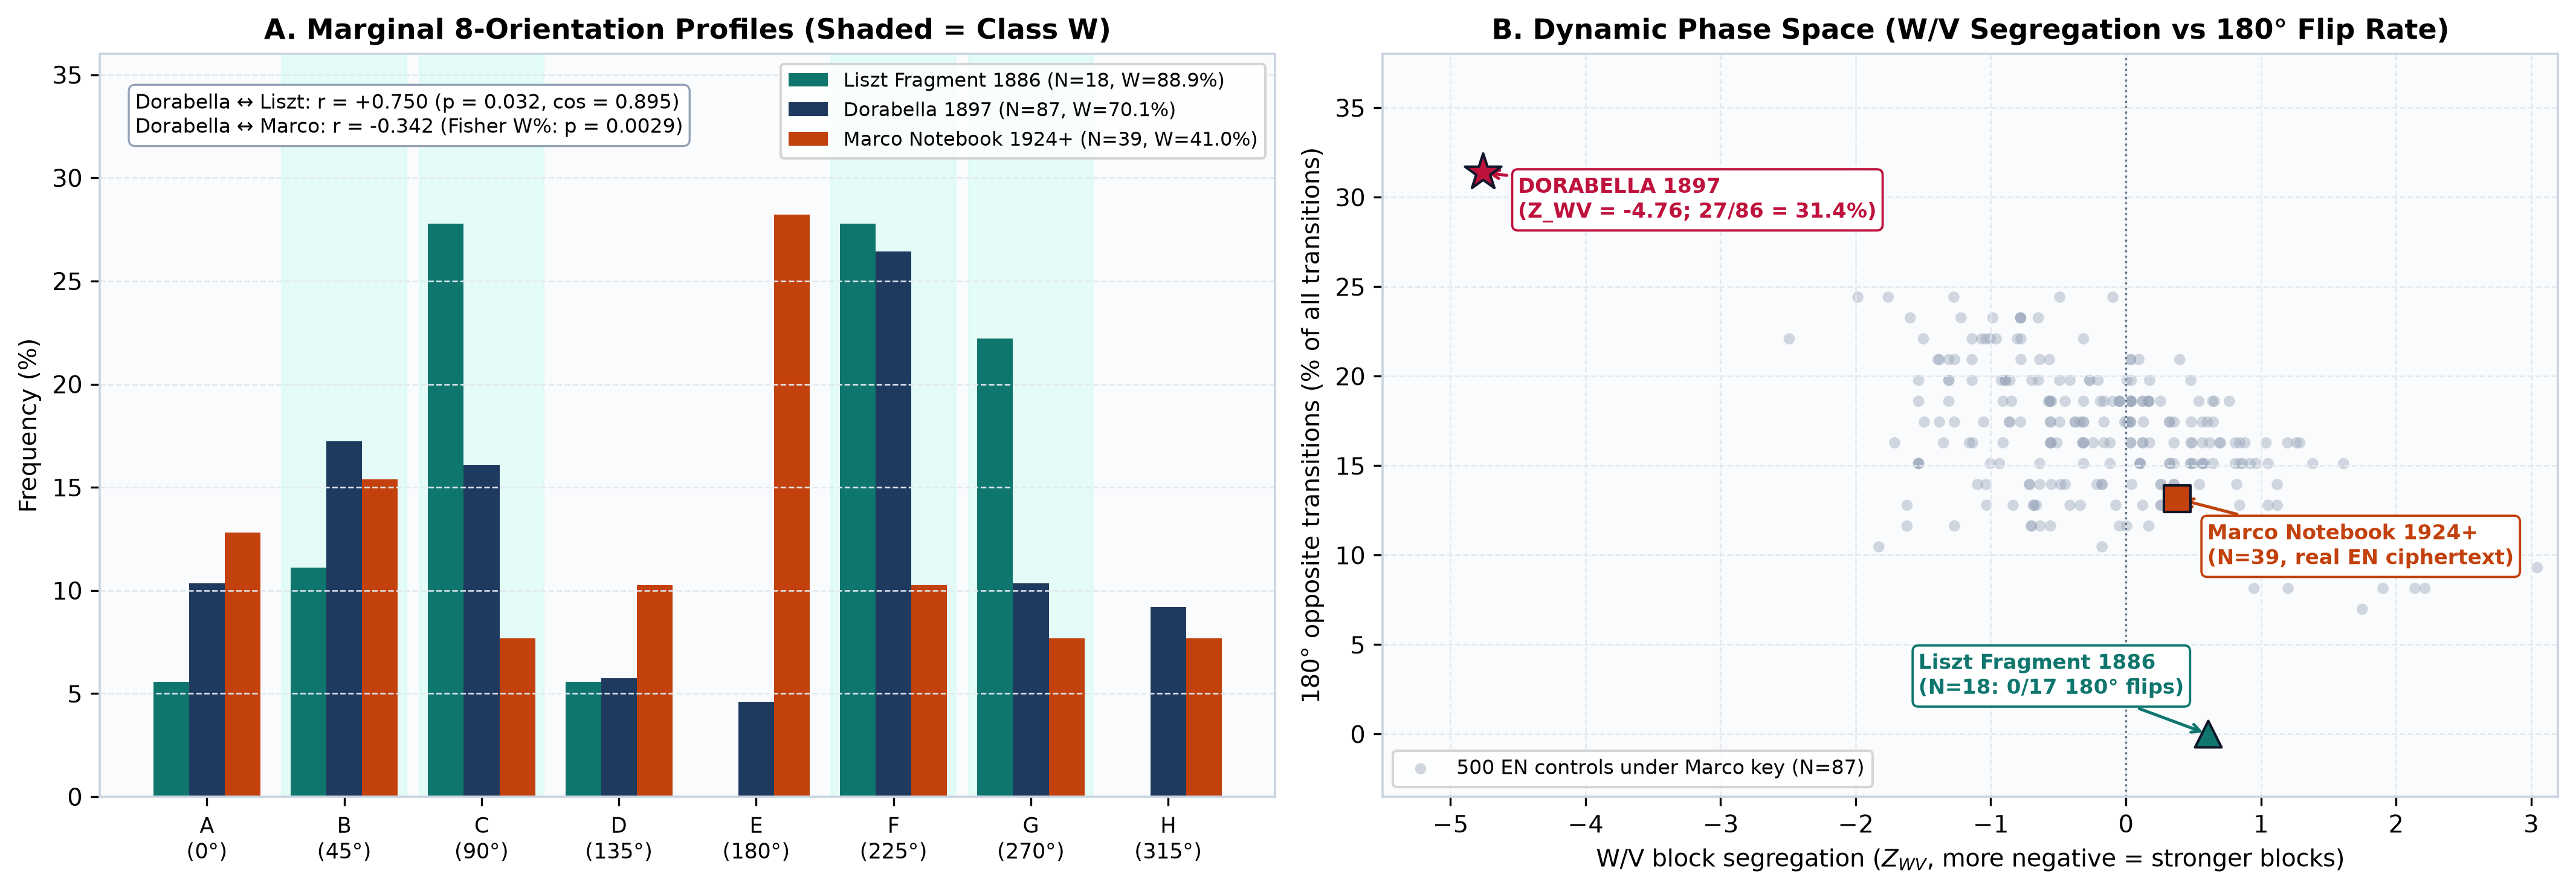
\includegraphics[width=\textwidth]{figures/fig3_en.png}
  \caption{Cross-corpus forensic comparison of Elgar's surviving semicircle documents. \textbf{(A)}~Marginal 8-orientation percentage profiles (shaded columns = class \code{W}): \emph{Liszt} (1886) and \emph{Dorabella} (1897) correlate closely ($r = +0.750$, $p = 0.032$), whereas \emph{Marco} (1924+) diverges ($r = -0.342$). \textbf{(B)}~Dynamic phase space ($Z_{WV}$ vs.\ $180^\circ$ flip rate): \emph{Dorabella} sits far outside the 500 Marco-key English controls ($0/500$ reach $Z_{WV} \le -4.76$ or $\ge 27$ $180^\circ$ flips), while \emph{Liszt} shows zero $180^\circ$ flips.}
  \label{fig:corpus}
\end{figure*}

Three forensic conclusions emerge:
\begin{enumerate}
  \item \textbf{Close marginal kinship between Liszt (1886) and Dorabella (1897):} Eleven years before Dorabella, Elgar's \emph{Liszt Fragment} exhibits the same unrotated 8-orientation profile ($r = +0.750$, two-tailed $p = 0.032$, one-tailed permutation $p = 0.020$, cosine $0.895$; sensitivity variant \code{Liszt\_alt}: $r = +0.768$, $p = 0.026$, cosine $0.911$), the same modal peak on \code{F}, matching nearly uniform arc counts ($\chi^2\,p = 0.881$), and a length-9 non-repeating-arc run. Assuming the archival authenticity of the \emph{Liszt Fragment} (housed at the Elgar Birthplace Museum \citep{bauer2017unsolved}, though \citet{ernst2018cipherbrain} also questioned its provenance), this 11-year marginal alignment provides \textbf{strong evidence rendering a 1937 fabrication by Dora Powell highly implausible}.
  \item \textbf{Sharp divergence from Elgar's verified English ciphertext (Marco 1924+):} The post-1924 notebook behaves like an ordinary English MASC ($Z_{WV} = +0.38$; $5/38$ $180^\circ$ flips vs.\ $5.13$ expected), with significantly lower \code{W} share ($41.0\%$; Fisher exact vs.\ Dorabella $p = 0.0029$, vs.\ Liszt $p = 0.0012$), uncorrelated orientations ($r = -0.342$), and 2-arc-heavy counts ($\chi^2$ vs.\ Dorabella $p = 0.023$). Among 500 English plaintexts ($N=87$) encrypted with the exact 1924 key, \textbf{$0/500$} reach $Z_{WV} \le -4.76$ and \textbf{$0/500$} reach $\ge 27$ $180^\circ$ flips.
  \item \textbf{Shared marginals, opposite dynamics:} While Elgar's preferred marginal repertoire (\code{W} dominance, peak \code{F}) is already present in 1886, \emph{Liszt} shows an opposite dynamic sign ($0/17$ $180^\circ$ flips, $Z = -2.19$). This marginal/dynamic dissociation is consistent with the same author producing two distinct genres---a brief marginal doodle vs.\ a playful, mirror-rich three-line letter---though $N=18$ limits strong dynamical inference on \emph{Liszt}.
\end{enumerate}

% =============================================================================
\section{Model Selection, Generative Adequacy, and 1D+2D Classification}
\label{sec:models}
% =============================================================================

\subsection{Leave-One-Out Cross-Validation on Transitions}
To compare dynamical hypotheses without overfitting, six transition models over the eight orientations were evaluated by exact leave-one-out cross-validation (LOO-CV) across the 86 orientation transitions of Dorabella (Table~\ref{tab:loocv} and Figure~\ref{fig:models}A). The 4-parameter calligraphic model (\code{W/V} posture persistence plus $180^\circ$ mirror reflex) achieves \textbf{$+12.03$~nats} over independence (Bayes factor $\approx 167{,}000:1$, perplexity $6.563$), beating both the 56-parameter full Markov chain ($+4.22$~nats) and the best-case \emph{a posteriori} 1D conjunct musical chain (\code{DHABFCGE}, $+3.43$~nats).

\begin{table}[t]
\centering
\caption{Out-of-sample LOO-CV across Dorabella's 86 orientation transitions (higher gain and lower perplexity are better).}
\label{tab:loocv}
\scriptsize
\setlength{\tabcolsep}{3pt}
\resizebox{\columnwidth}{!}{%
\begin{tabular}{@{}lccc@{}}
\toprule
\textbf{Transition Model} & \textbf{Params} & \textbf{$\Delta$ vs.\ IID} & \textbf{Ppl.} \\
\midrule
0. IID (smoothed marginals)      & $+0$  & $0.00$ nats   & 7.548 \\
2. $180^\circ$ mirror reflex only & $+1$  & $+6.19$ nats  & 7.024 \\
5. Full smoothed $8\times 8$ Markov & $+56$ & $+7.81$ nats  & 6.893 \\
1. Optimal 1D musical chain      & $+1$  & $+8.59$ nats  & 6.831 \\
3. \code{W/V} posture blocks only & $+2$  & $+8.98$ nats  & 6.799 \\
\textbf{4. \code{W/V} + $180^\circ$ mirror} & \textbf{$+4$} & \textbf{$+12.03$ nats} & \textbf{6.563} \\
\bottomrule
\end{tabular}}
\end{table}

\subsection{Descriptive Generative Adequacy (500 Simulations)}
To test whether candidate mechanisms can jointly reproduce Dorabella's 2D profile, we simulated 500 87-glyph realizations from five full $(o,a)$ generators, incorporating 272 authentic Elgar melody notes (\emph{Enigma Theme}, \emph{Variation X ``Dorabella''}, \emph{Salut d'Amour}, \emph{Chanson de Matin}, \emph{Pomp and Circumstance No.~1} Trio; Table~\ref{tab:gen} and Figure~\ref{fig:models}B). Because \code{G2} is calibrated directly to Dorabella's empirical dynamics (5 dynamic scalars---\code{p\_stay\_w}, \code{p\_stay\_v}, \code{p\_flip\_same}, \code{p\_flip\_diff}, \code{anti\_rep}---plus 2 mild drift slopes and 4 axis-symmetric arc priors), we treat Table~\ref{tab:gen} strictly as a \textbf{descriptive adequacy check}, relying on Section~5.1 (LOO-CV) and Section~5.3 (uncalibrated prior classification) for non-circular predictive tests.

\begin{figure*}[t]
  \centering
  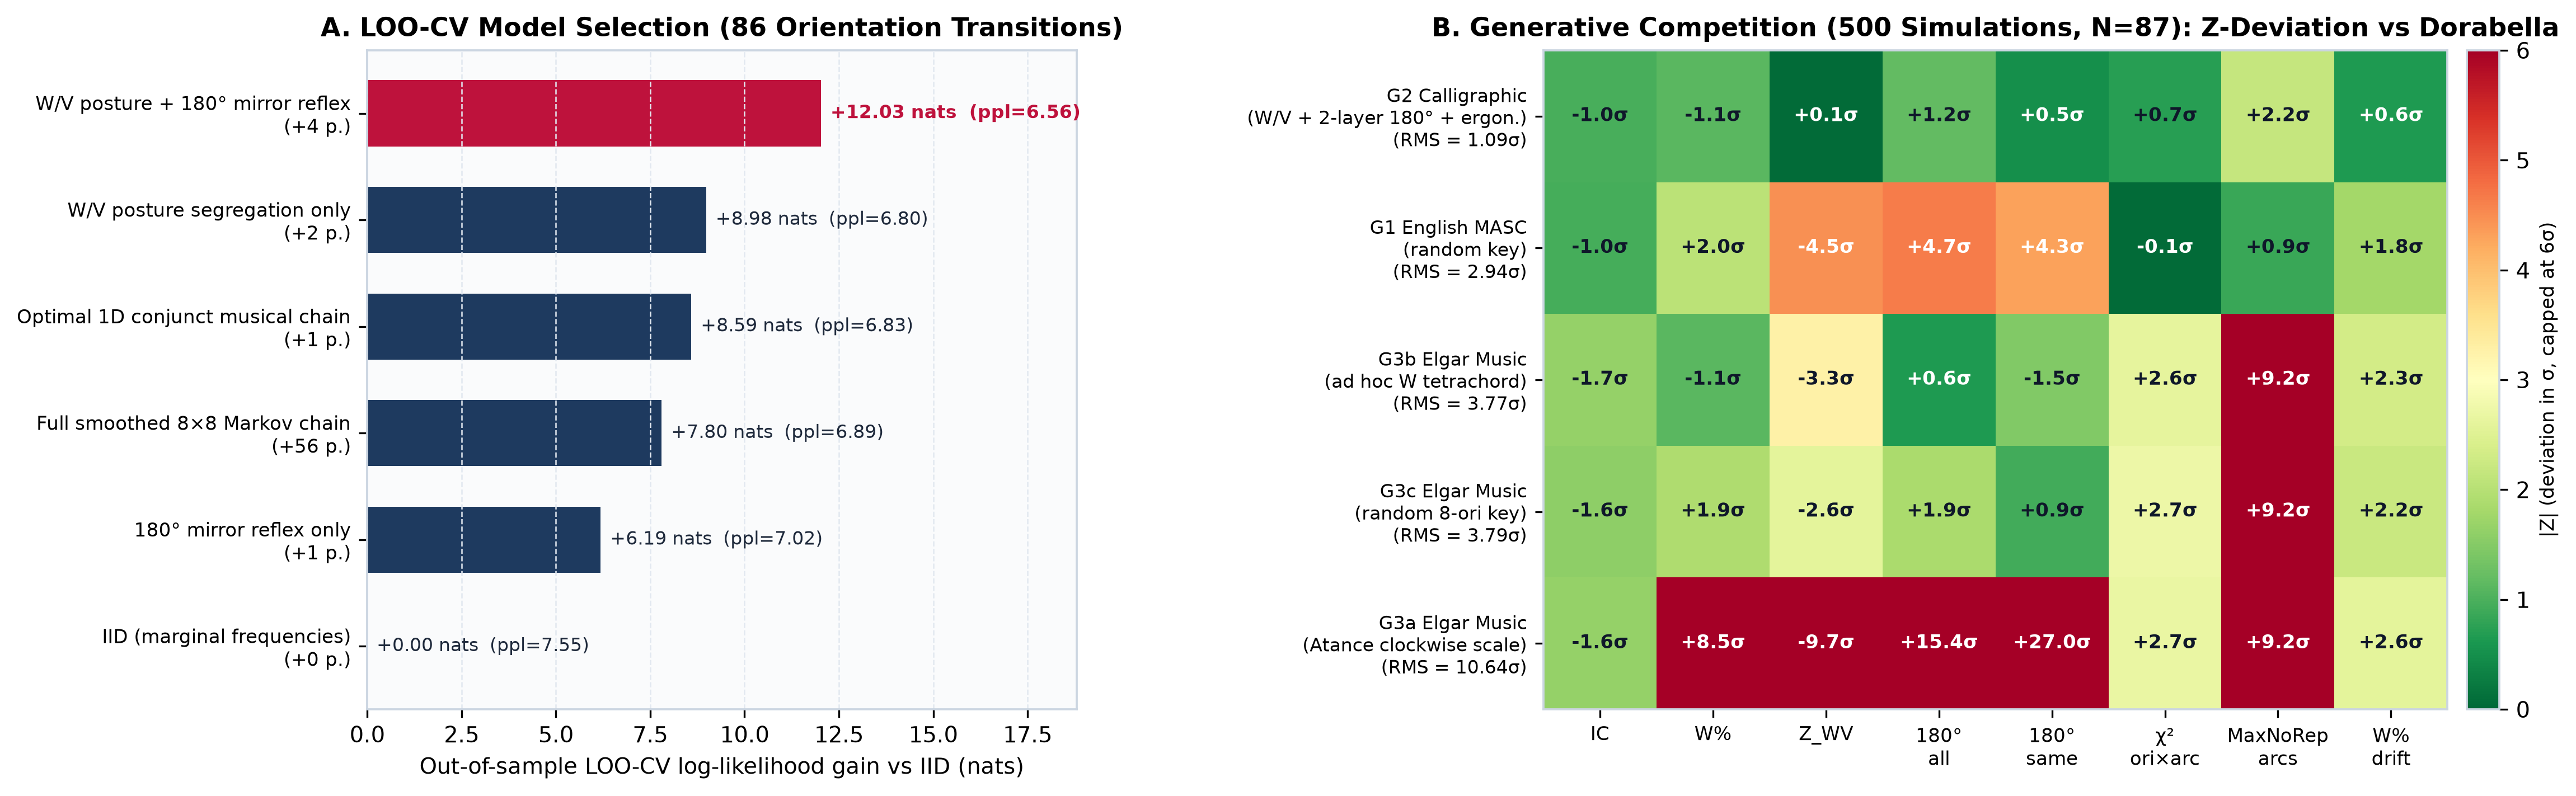
\includegraphics[width=\textwidth]{figures/fig4_en.png}
  \caption{\textbf{(A)}~Out-of-sample LOO-CV log-likelihood gain over IID across the 86 orientation transitions: the 4-parameter calligraphic model dominates all competitors ($+12.03$~nats). \textbf{(B)}~Descriptive generative adequacy (500 simulations per model, $N=87$): signed $Z$-deviations from Dorabella across eight structural metrics, ordered by RMS error.}
  \label{fig:models}
\end{figure*}

\begin{table*}[t]
\centering
\caption{Descriptive generative adequacy (500 simulations of $N=87$ per model) against observed Dorabella metrics (signed $Z$-deviations in parentheses). Musical models test direct pitch-by-orientation + rhythm-by-arc mappings on five authentic Elgar themes.}
\label{tab:gen}
\footnotesize
\setlength{\tabcolsep}{3.6pt}
\resizebox{\textwidth}{!}{%
\begin{tabular}{@{}lccccccccc@{}}
\toprule
\textbf{Generative Model ($N=87$)} & \textbf{IC} & \textbf{\code{W}\%} & \textbf{$Z_{WV}$} & \textbf{$180^\circ$ all} & \textbf{$180^\circ$ same} & \textbf{$\chi^2_{OA}$} & \textbf{MaxNoRep} & \textbf{\code{W}\% drift} & \textbf{RMS $|Z|$} \\
\midrule
\textbf{DORABELLA (1897, obs.)} & \textbf{0.0585} & \textbf{70.1\%} & \textbf{$-4.76$} & \textbf{27} & \textbf{13} & \textbf{40.2} & \textbf{13} & \textbf{$+22.9\%$} & \textbf{0.00$\sigma$} \\
\textbf{\code{G2} Calligraphic (calibrated)} & 0.0692 & 79.0\% & \textbf{$-4.82$} ($+0.1\sigma$) & 22.2 ($+1.2\sigma$) & 11.4 ($+0.5\sigma$) & 33.0 ($+0.7\sigma$) & 8.1 ($+2.2\sigma$) & $+10.8\%$ & \textbf{1.09$\sigma$} \\
\code{G1} English MASC (rand.\ key) & 0.0641 & 50.7\% & $+0.18$ (\textbf{$-4.5\sigma$}) & 10.8 (\textbf{$+4.7\sigma$}) & 3.6 (\textbf{$+4.3\sigma$}) & 40.9 & 10.3 & $+0.7\%$ & 2.94$\sigma$ \\
\code{G3b} Elgar Music (ad hoc \code{W}) & 0.0808 & 72.2\% & $-1.44$ (\textbf{$-3.3\sigma$}) & 24.6 & 16.9 & 21.2 & \textbf{4.8} (\textbf{$+9.2\sigma$}) & $-0.3\%$ & 3.77$\sigma$ \\
\code{G3c} Elgar Music (rand.\ key) & 0.0797 & 50.0\% & $+1.37$ & 12.2 & 7.7 & 21.3 & \textbf{4.8} (\textbf{$+9.2\sigma$}) & $+0.7\%$ & 3.79$\sigma$ \\
\code{G3a} Elgar Music (clockwise) & 0.0804 & 54.3\% & $+1.83$ (\textbf{$-9.7\sigma$}) & 3.1 (\textbf{$+15.4\sigma$}) & 0.3 (\textbf{$+27.0\sigma$}) & 20.9 & \textbf{4.8} (\textbf{$+9.2\sigma$}) & $+0.1\%$ & \textbf{10.64$\sigma$} \\
\bottomrule
\end{tabular}}
\end{table*}

While \code{G2} fits Dorabella cleanly ($\mathrm{RMS}=1.09\sigma$), it still slightly under-predicts \code{MaxNoRep} ($8.1$ vs.\ $13$, $+2.2\sigma$), indicating a residual opening-line arc-variation habit not yet modeled. English MASC (\code{G1}, $2.94\sigma$) fails severely on \code{W/V} ($-4.5\sigma$) and $180^\circ$ flips ($+4.7\sigma/+4.3\sigma$). Within the tested class of \textbf{direct pitch-by-orientation + rhythm-by-arc encodings}, musical models fail catastrophically: clockwise mapping (\code{G3a}) reaches $10.64\sigma$, and even an \emph{ad hoc} \code{W}-tetrachord mapping (\code{G3b}, $3.77\sigma$) fails on rhythm (\code{MaxNoRep} $= 4.8$ vs.\ $13$, $+9.2\sigma$); more abstract interval/contour or alternative rhythmic encodings remain outside the tested class. Note also that inter-line \code{W} drift (L1 $58.6\%$ $\to$ L2 $71.0\%$ $\to$ L3 $81.5\%$) is not significant on $N=87$ ($\chi^2 = 3.50$, $p = 0.173$; Spearman $\rho = +0.167$, $p = 0.122$) and is treated strictly as descriptive.

\subsection{Resolving Foxon's 1D Boundary: 1D vs.\ 1D+2D Classification}
Directly answering \citet{foxon2025ml}'s call for new discriminating features, we trained RBF-SVM and MLP classifiers (5-fold CV, 800 samples/class) separating real English MASCs ($N=87$) from a \textbf{broad, uncalibrated prior family} of 2D calligraphic pseudo-ciphers (randomized per-sample posture persistence, mirror rates, and Dirichlet axis-symmetric arc priors---zero point-parameter leakage from Dorabella), comparing 12 permutation-invariant 1D features against \textbf{1D + our 4 2D features} ($\min Z_{WV}$, all-arc and same-arc $180^\circ$ flip rates, $\cos_{180^\circ}$; Table~\ref{tab:foxon}).

\begin{table}[t]
\centering
\caption{Foxon-style 1D vs.\ 1D+2D hoax-detection benchmark (5-fold CV and out-of-sample probabilities $P(\text{English MASC})$). Marco ($N=39$) is evaluated on a length-matched $N=39$ model.}
\label{tab:foxon}
\scriptsize
\setlength{\tabcolsep}{3pt}
\resizebox{\columnwidth}{!}{%
\begin{tabular}{@{}lcccc@{}}
\toprule
\textbf{Evaluation Target / CV Metric} & \multicolumn{2}{c}{\textbf{RBF-SVM}} & \multicolumn{2}{c}{\textbf{MLP Neural Net}} \\
\cmidrule(lr){2-3}\cmidrule(lr){4-5}
& \textbf{1D only} & \textbf{1D+2D} & \textbf{1D only} & \textbf{1D+2D} \\
\midrule
5-fold CV Accuracy ($N=87$)      & 93.4\% & \textbf{99.94\%} & 93.4\% & \textbf{99.94\%} \\
5-fold CV ROC-AUC ($N=87$)       & 0.9821 & \textbf{0.9999}  & 0.9761 & \textbf{0.9999}  \\
\midrule
\code{Dorabella} (\code{Hauer\_2025})     & 0.7724 & \textbf{0.0008}  & 0.9728 & \textbf{0.0016}  \\
\code{Dorabella} (\code{Hartmeier\_2017}) & 0.7724 & \textbf{0.0008}  & 0.9790 & \textbf{0.0021}  \\
\code{Dorabella} (\code{Pelling\_2012})   & 0.7805 & \textbf{0.0013}  & 0.9446 & \textbf{0.0015}  \\
\midrule
\emph{Marco Notebook} (1924+, $N=39$, EN) & 0.7422 & \textbf{1.0000}  & 0.9929 & \textbf{1.0000}  \\
\bottomrule
\end{tabular}}
\end{table}

Table~\ref{tab:foxon} reproduces and resolves \citet{foxon2025ml}'s paradox cleanly: in 1D alone, Dorabella scores $P(\text{English}) = 0.772$ (SVM) and $0.973$ (MLP). Adding our four 2D features lifts CV accuracy to \textbf{99.94\%} and flips Dorabella instantaneously to \textbf{$P(\text{English}) \le 0.0021$} ($>99.79\%$ 2D Calligraphic across all three transcriptions), while Elgar's genuine \emph{Marco Notebook} ciphertext ($N=39$, length-matched control) moves in the \emph{opposite} direction to \textbf{$P(\text{English}) = 1.0000$} on both classifiers.

% =============================================================================
\section{Discussion, Epistemic Scope, and Conclusion}
\label{sec:discussion}
% =============================================================================

Restoring the 2D geometry of Dorabella's glyphs resolves the tension between MASC solver failure \citep{hauer2021dorabella,wase2025dorabella} and 1D classifier ambiguity \citep{foxon2024ann,foxon2025ml}. Four reproducible, empirically weakly correlated 2D findings---(1)~\code{W/V} posture blocking ($Z = -4.76$, $0/1{,}000$ EN MASCs), (2)~two-layer $180^\circ$ flips ($48.1\%$ same-arc within fixed \code{W/V}, $p = 0.0012$; $0/1{,}000$ EN MASCs), (3)~$180^\circ$ ergonomic arc-profile symmetry (rank \#1/105; $1/1{,}000$ EN MASCs; $0/1{,}000$ jointly), and (4)~cross-corpus kinship with \emph{Liszt} (1886) versus divergence from \emph{Marco} (1924+)---converge on an \textbf{improvised calligraphic pseudo-cipher or playful graphic joke written by Elgar himself in 1897}.

Following \citet{foxon2024ann}'s caution regarding the Zodiac Z340 cipher, statistical evidence cannot establish deductive impossibility. Rather, these invariants define a falsifiable quantitative benchmark: any future decipherment proposal---linguistic, steganographic, or musical---must simultaneously account for $Z_{WV} = -4.76$, the \#1/105 $180^\circ$ arc-profile symmetry, and the $48.1\%$ same-arc $180^\circ$ mirror reflex.

\paragraph{Reproducibility \& AI Assistance Disclosure.} All datasets, deterministic scripts (fixed seeds), figures, and prior refutation audits reproduce end-to-end via \code{python3 scripts/reproduce\_all.py}. Computational implementation, statistical simulations, and LaTeX drafting assistance were carried out using \textbf{Arena.ai Agent Mode} under the direction, critical auditing, and full scientific responsibility of the author (Christophe Marcheux).

\bibliographystyle{plainnat}
{\scriptsize\setlength{\bibsep}{0.6pt}\bibliography{references}}

\end{document}
